%%%%%%%%%%%%%%%%%%%%%%%%%%%%%%%%%%%%%%%%%%%%%%%%%%%%%%%%%%%%%%%%%%
%%%%%%%% ICML 2012 EXAMPLE LATEX SUBMISSION FILE %%%%%%%%%%%%%%%%%
%%%%%%%%%%%%%%%%%%%%%%%%%%%%%%%%%%%%%%%%%%%%%%%%%%%%%%%%%%%%%%%%%%

% Use the following line _only_ if you're still using LaTeX 2.09.
%\documentstyle[icml2012,epsf,natbib]{article}
% If you rely on Latex2e packages, like most moden people use this:
\documentclass{article}

% For figures
\usepackage{graphicx} % more modern
%\usepackage{epsfig} % less modern
\usepackage{subfigure} 
\usepackage{enumitem}
% For citations
\usepackage{natbib}

% For algorithms
\usepackage{algorithm}
\usepackage{algorithmic}

% As of 2011, we use the hyperref package to produce hyperlinks in the
% resulting PDF.  If this breaks your system, please commend out the
% following usepackage line and replace \usepackage{icml2012} with
% \usepackage[nohyperref]{icml2012} above.
\usepackage{hyperref}

% Packages hyperref and algorithmic misbehave sometimes.  We can fix
% this with the following command.
\newcommand{\theHalgorithm}{\arabic{algorithm}}

% Employ the following version of the ``usepackage'' statement for
% submitting the draft version of the paper for review.  This will set
% the note in the first column to ``Under review.  Do not distribute.''
\usepackage{icml2012} 
% Employ this version of the ``usepackage'' statement after the paper has
% been accepted, when creating the final version.  This will set the
% note in the first column to ``Appearing in''
% \usepackage[accepted]{icml2012}


% The \icmltitle you define below is probably too long as a header.
% Therefore, a short form for the running title is supplied here:
\icmltitlerunning{Submission and Formatting Instructions for ICML 2012}



\begin{document} 

\twocolumn[
\icmltitle{Sentiment Extraction of Earbud Amazon Reviews }

\icmlkeywords{boring formatting information, machine learning, ICML}

\vskip 0.3in
]

\section{Introduction}
Amazon.com provides an abundant amount of reviews to aid buyers on their decision to purchase the product. However, it is very time consuming for buyers to read through all the reviews and filter through them for only information relevant to them. Although Amazon attempts
to ease the problem by ranking its reviews in order of helpfulness, the top reviews may only be considered a top review simply due to visibility. To solve this issue, we propose to automatically extract sentiments from the entire set of reviews and aggregate it in a concise summary.

Our basic approach is to first generate a word bank of relevant terms using LDA from the product descriptions and questions asked by purchasers on the product. Next, using SVM and SentiWordNet with Word Sense Disambiguation (WSD), annotated all sentences with a sentiment score and only use the non-neutral sentences in the n-gram generator to produce relevant adj-noun bigrams or trigrams. These terms will be filtered by the word bank produced by the LDA and ranked to produce a set of most relevant terms with their sentiment. The output will be terms that our algorithm decides to be the most relevant. 


\section{Problem Definition and Methods} 
 \subsection{Task Definition}
Our problem is to extract sentiment tagged aspects that will give a good representation of the text corpus it was generated from using the method described below. The main questions we want to answer are:
\begin{enumerate}
\item What are characteristics of products important to consumers?
\item What are important features reviewers focus on?
\item What makes review content irrelevant or less relevant?
\end{enumerate}

It is an important problem, because accurate extraction of sentiment would save consumers lots of time in any e-commerce market place setting which relies on large numbers of product reviews to sway consumers to purchase a product. What we are proposing is an algorithm that can be applied to any product because it adapts to be context specific through analysis of prior information for each product. Furthermore, this can be applied to other areas involving text summarization, such as automated generation of catch phrases and key points for company ads
\subsection{Algorithm and Methods}
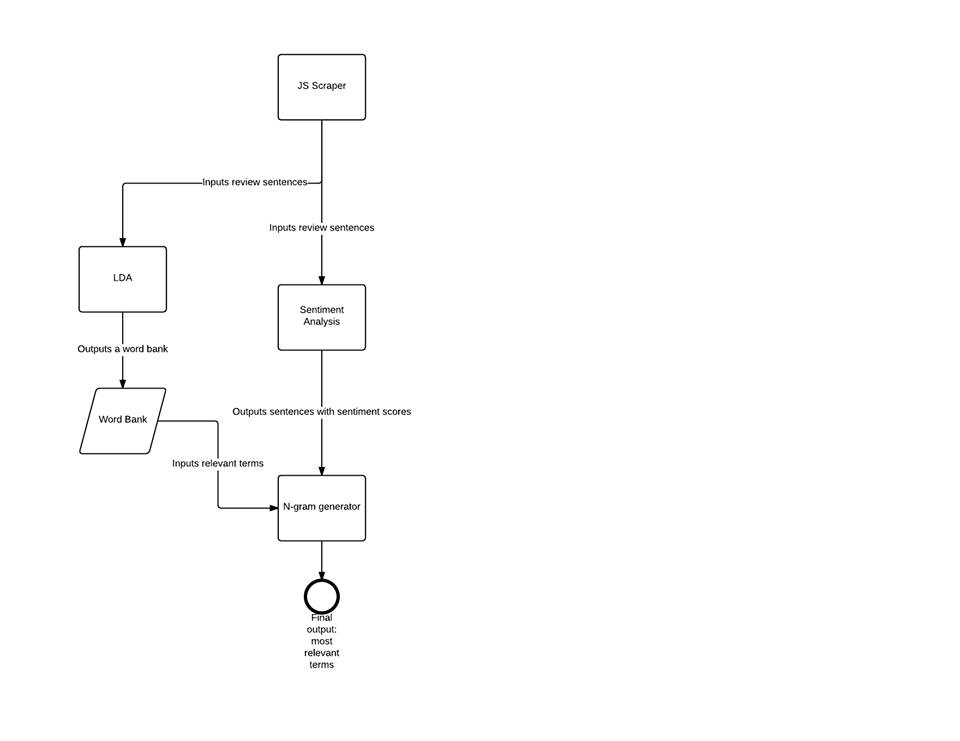
\includegraphics{flow.jpg}
Given one of the research questions is to understand what product features and terms are relevant to a prospective consumer. The goal is to be able to have contextual terms that will refine the results of the n-gram generator by using prior information provided for the products. In this case we used product descriptions that we mined to form a corpus of documents which describe different earbuds/headphones products. 

In previous works, it has been shown that LDA can be used as an effective unsupervised learning algorithm to cluster textual data into a series of highly probable topics that describe the corpus' contents. We chose LDA as it can run unsupervised and uses a generative model to determine what topics comprise the corpus of documents and how those topics can be described with certain text terms. In terms of the problem statement, this provides us with a basic understanding of the terms that product sellers believe is relevant to a consumer. The assumptions made include that the terms in the product description actually have some form of relevancy to the general products in the earbuds category. This is justified by the assumption that these product descriptions are formed based on the market research the product seller has done. This approach ignores the possibilities that certain terms are relevant to different classes of earbuds, and that the seller may have misinterpreted the interests of the consumer.

Our process is as follows. We collected a large set of product descriptions we manually mined from a variety of different product pages on Amazon. We set each description to represent a document. We used the standard stopword filter to filter out words that are usually considered irrelevant when analyzing text. We then run a version of unsupervised LDA which takes in a set of documents, a stopword list and the number of topics that we want to extract. We utilized a k value equal to fifteen and ran the LDA in six different runs where each run ran LDA either fifty times or two-hundred fifty iterations. Using the results from the six runs we can corroborate that similar terms are extracted from each run implying that the terms are considered all interrelated and also relevant. This is necessary as LDA is a probabilistic model so different runs can extract different topics, however we believe that iterating on these independent runs can still lead to the extraction of similar tone/word topics. Through this, we hope to create a word bank of terms that are contextually related to the main product. We can use these terms as a resource when ranking the sentiments extracted, and filtering based on a relevancy threshold.  

To extract relevant terms from the reviews, each sentence of the reviews was made into a POS-tagged parse tree and chunked on various grammars. Through multiple runs of chunking on different grammars, it was determined that chunking into bigrams of <adj>*<noun>* and trigrams of <DT>?<adj>*<noun>* were most accurate in extracting relevant terms. To offset the thousands of false positives the parse tree generated, the results of the parse tree were filtered by the word bank generated by the LDA. If the word existed in the LDA, it would be given heavier weight. At the end, only words with a weight above a certain threshold were considered relevant terms. 

To give each sentence a sentiment score, we first train a bag of words with a combination of the movie review corpus from nltk and a portion of the annotated laptop reviews from Stanford SNAP library with all the unique words stemmed by using Porter Stemmer. With an interface to SentiWordNet using the NLTK WordNet classes, for each sentence, we split it into individual words and for each word in that sentence, we look it up in the SentiWordNet dictionary for its positive and negative sentiment scores. SentiWordNet is a document recourse which contains a list of English terms which have been attributed a score of positivity and negativity. By using the sentiment scores from SentiWordNet, we can make an educated prediction of the sentence’s expressed sentiment. 

In order to obtain more accurate results, we also implemented WSD(Word Sense Disambiguation) and found the closest meaning of a given word w through the maximum path similarity of w and the other words in the sentence. The sentiment score of a sentence would be the summation of the weighted sentiment scores of the words inside that sentence. By weighted, we mean if this word appeared more times in the positive class, its positive sentiment score is multiplied by the log of its frequency in the positive class. If a word does not exist in the bag of words we obtained from training, it will simply be ignored.

To score each sentence with SVM, we use the annotated laptop reviews to create feature vectors representing word counts for each word encountered in the training data. The soft margin weight vector is then computed using SVMlight. This weight vector is used to assign a sentiment score to each sentence. 

\section{Experimental Evaluation} 
\subsection{Methodology}
\begin{enumerate}
\item Preprocessing stage: 
\newline Using the scraper extract all user reviews and split by sentence to generate a list of sentences from all the reviews per product.

\item Processing stage
	\begin{enumerate} [label* = \arabic*.]
	\item Determining Important Features of each product \\
	This will be done with a combined static and dynamic technique.
		\begin{enumerate} [label* = \arabic*.]
	\item Static Technique \\
	 Generate important aspects from product descriptions scraped from Amazon.com by using an LDA analysis. These words, along with the words sound, audio, comfort, bass, highs, mids, tones, durability, quality, blocking, noise, sharp, deep, and tangle will be considered important aspects automatically and provide a way to weight sentences based on perceived relevancy to the product domain of earbuds.
	\item Dynamic Technique \\
	 Using a parse tree split each sentence into bigrams and trigrams with the grammar format of $<$adj$><$noun$>$ to represent candidate product aspects of importance to reviewers. We can filter this list using stopword filters and other grammatical based rules to get rid of false positives. We can create an inverted index of these terms and the sentences they occurred in. We can also easily use the list of sentences to find the frequency of aspects in the review corpus.
	\end{enumerate}
		\item Using SVM or Naive Bayes annotate each sentence with a sentiment score based on the previously created list of relevant features for the product. If a sentence has a score below a low threshold then it will be discarded.
	\end{enumerate}
\item Post-processing stage: Aggregation
	\begin{enumerate}[label* = \arabic*.]
	\item We need to summarize the aspect information we have and present sentences from the corpus that best represent the corpus. One way to do this is to rank the aspects based on frequency and then calculate an averaged sentiment score, which can be used to determine which sentiment polarity the majority of the reviews have with respect to that aspect. We can then take a sentence to represent this aspect. A simple scheme could be to find the sentence with the greatest magnitude sentiment score with the same polarity as the aspect average score.
	\end{enumerate}
\end{enumerate}
We believe the main problem can be solved through a composition of the above techniques to filter neutral sentiments, extract entities that may describe the product, rank the entities based on relevancy to product, followed by ranking the sentiments based on frequency of occurrence or aggregate sentiment towards a given entity.  

The reasoning behind this is that the problem seeks to extract sentiments. A sentiment is defined as an author’s opinion (positive or negative) about a given product feature (herein referred to as an aspect). We must first filter neutral sentiments which likely have factual information rather than opinions.

Next we seek to do a form of entity extraction using the n-gram generator so as to have a list of potential aspects that are being referenced in the sentence. These aspects could be potential targets of the sentence’s sentiment. This naively ignores the possibility of compound sentiment where there may be multiple sentiments with different targets. We justify this through the assumption most reviews usually spread their evaluation over a variety of areas and analyze each one individually.

Following the entity extraction which is based entirely on structural information in the sentence and POS tagging, we use contextual information to determine what is relevant to the product. Given the same exact review for a headphone product, an iPhone product, and a guitar product, the focus of what entities are relevant to the consumer will change. However using our LDA analysis we can ensure we only utilize the aspects consumers are most likely to be interested in.

To evaluate our results, we ran the different parts of our algorithm on laptop review data that was annotated with relevant terms per sentence and each of those terms was annotated with either “positive”, “negative”, or “neutral” sentiment. Since we wanted to get the overall sentiment of the sentence, each sentence was given a sentiment score based on majority vote of the sentiment of the terms extracted from it. The testing and training data are realistic, because it is also technology review data that focused on extraction of relevant terms and sentiment as a mean of text summarization. 

Each part of the algorithm was benchmarked using annotated data to get accuracy of the individual parts. Our goal is to determine if we can answer the research questions using the components described for the overall goal of extracting relevant sentiments. We benchmarked them separately and evaluated them based on their performance at their individual task.

At the moment there is no effective way for us to evaluate the relevancy of the outputted sentiments, though theoretically it could be evaluated through the construction of an information retrieval problem where we try to see how relevant the top sentiments are to a corpus of consumer submitted questions on Amazon.

In order to determine if a review sentence is opinionated, we need to be able to apply sentiment analysis on each input sentence. We decided to experiment with two different approaches to see which one would have a better performance in terms of correctly classifying each sample. 

One of the two approaches was using SentiWordNet and WSD to train and test a sentiment classifier on the annotated laptop reviews. Since only the opinionated sentences were relevant to our project and that SentiWordNet only supports a binary classification of either positive or negative, all the “neutral” data samples were ignored, which left us with 1220 annotated sentences. The sentences had aspect terms marked for each of them, and each aspect term had a sentiment. We simply took the majority vote on the sentiment of the overall sentence based on the sentiments of the aspect terms. The algorithm works as described in section 2.2, and we tested it with a 4-fold cross validation methodology in which each fold included 70\% of the samples used as training data and the other 30\% used as testing data. The accuracies were obtained by checking the classification produced by our algorithm against the assigned sentiment of the sentence from applying majority vote on its aspect terms’ sentiments. Below are the results:

The algorithm for extracting relevant terms from the parse tree was run multiple times using different grammars to chunk on in order to determine which grammar produced the most accurate results. In general, the tree chunked on adj ,noun bigrams or determiner,adj,noun trigrams. The results were checked against the annotated laptop review data we obtained. Majority of the review sentences in that dataset have aspect terms marked, so we checked the bigrams and trigrams produced by our n-gram generator to see if our results matched the annotated aspect terms of that sentence. The results are summarized below: 


\subsection{Results}

\subsection{Discussion}
The high amount of false positives in term selection via parse tree chunking on bigrams and trigrams is due to the oversensitivity of the chunker. The parse tree will chunk on any phrase that fulfills the grammar, including terms such as “father” or “mother”, which are nouns but irrelevant to the reviews. This implies having contextual information is important and can benefit the n-gram generator. This also implies basic grammar chunkings may not be optimal and more specific grammars may need to be utilized.
\section{Related Work}
We will restrict our focus to one type of product (headphones) to make evaluation easier. We see 3 main stages to this project:





\section{Future Work}
\section{Conclusion}
\section{Resources}

Python libraries: Sci-Kit Learn, NLTK, Numpy, Scipy

Data for benchmarking and testing accuracy

\begin{itemize}
\item Web scraper written in Node.js to parse relevant data (reviews, product descriptions, etc)
\newline 

\item Annotated data from SemEval2014-Task4 on aspect feature based sentiment analysis
\newline
\url{http://alt.qcri.org/semeval2014/task4/index.php?id=data-and-tools}

\item Amazon product review data mined by Stanford
\newline
\url{http://snap.stanford.edu/data/web-Amazon-links.html}
\end{itemize}

Readings on Parsing \& Sentiment Analysis:
\begin{itemize}
\item Stanford paper on parsing \& sentiment analysis:
\newline
\url{http://nlp.stanford.edu/~socherr/EMNLP2013_RNTN.pdf}

\item Multi-aspect sentiment analysis
\newline 
\url{http://www.cs.cornell.edu/home/cardie/papers/masa-sentire-2011.pdf}

\item Catching the Drift: Probabilistic Content Models, with Applications to
Generation and Summarization \newline
\url{http://www.aclweb.org/anthology/N04-1015}
\end{itemize}


\end{document}